\let\negmedspace\undefined
\let\negthickspace\undefined
\documentclass[journal]{IEEEtran}
\usepackage[a5paper, margin=10mm, onecolumn]{geometry}
%\usepackage{lmodern} % Ensure lmodern is loaded for pdflatex
\usepackage{tfrupee} % Include tfrupee package

\setlength{\headheight}{1cm} % Set the height of the header box
\setlength{\headsep}{0mm}     % Set the distance between the header box and the top of the text

\usepackage{gvv-book}
\usepackage{gvv}
\usepackage{cite}
\usepackage{amsmath,amssymb,amsfonts,amsthm}
\usepackage{algorithmic}
\usepackage{graphicx}
\usepackage{textcomp}
\usepackage{xcolor}
\usepackage{txfonts}
\usepackage{listings}
\usepackage{enumitem}
\usepackage{mathtools}
\usepackage{gensymb}
\usepackage{comment}
\usepackage[breaklinks=true]{hyperref}
\usepackage{tkz-euclide} 
\usepackage{listings}
% \usepackage{gvv}                                        
\def\inputGnumericTable{}                                 
\usepackage[latin1]{inputenc}                                
\usepackage{color}                                            
\usepackage{array}                                            
\usepackage{longtable}                                       
\usepackage{calc}                                             
\usepackage{multirow}                                         
\usepackage{hhline}                                           
\usepackage{ifthen}                                           
\usepackage{lscape}
\usepackage{circuitikz}
\tikzstyle{block} = [rectangle, draw, fill=blue!20, 
    text width=4em, text centered, rounded corners, minimum height=3em]
\tikzstyle{sum} = [draw, fill=blue!10, circle, minimum size=1cm, node distance=1.5cm]
\tikzstyle{input} = [coordinate]
\tikzstyle{output} = [coordinate]


\begin{document}

\bibliographystyle{IEEEtran}
\vspace{3cm}

\title{1.5.1}
\author{EE25BTECH11013 - Bhargav}
\maketitle
% \newpage
% \bigskip
{\let\newpage\relax\maketitle}

\renewcommand{\thefigure}{\theenumi}
\renewcommand{\thetable}{\theenumi}
\setlength{\intextsep}{10pt} % Space between text and floats


\numberwithin{equation}{enumi}
\numberwithin{figure}{enumi}
\renewcommand{\thetable}{\theenumi}

\textbf{Question}:\\
The center of a circle whose endpoints of a diameter of the circle A, B are \brak{-6,3} and \brak{6,4} is\\ 
\solution \\
Let the endpoints of the diameter of the circle be $\vec{A}$ and $\vec{B}$:
\begin{align}
    \vec{A}=\myvec{$-6$ \\ $3$},\quad
    \vec{B}=\myvec{$6$ \\ $4$}
\end{align}
We can use the midpoint formula to find the center of the circle.\\ 
The center $\vec{C}$ is the midpoint of $\vec{A}$ and $\vec{B}$: \\



\begin{align}
    \vec{C}=\frac{\vec{A}+\vec{B}}{2} 
\end{align}
\begin{align}
    \vec{C}=\frac{1}{2}\myvec{-6+6 \\ 3+4} 
\end{align}
\begin{align}
    \vec{C}=\frac{1}{2} \myvec{0 \\ 7} 
\end{align}
\begin{align}
    \vec{C}=\myvec{0\\\tfrac{7}{2}}.
\end{align}
\\
From the figure, it is clearly verified that the theoretical solution matches with the computational solution.\\
\begin{figure}[h!]
    \centering
    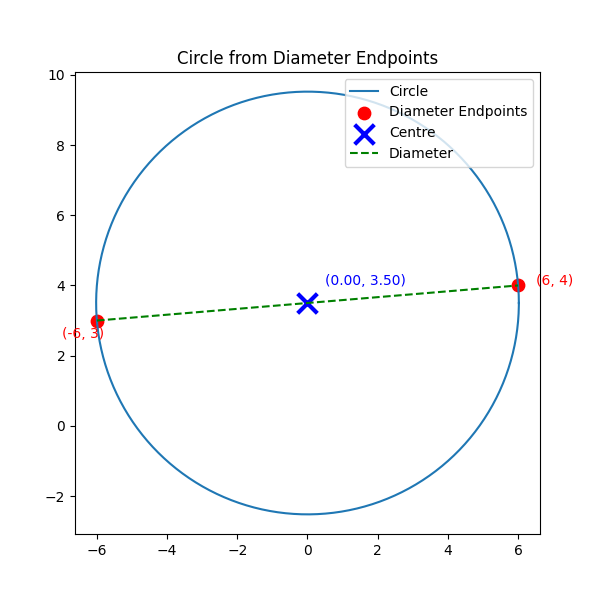
\includegraphics[height=0.5\textheight, keepaspectratio]{figs/Figure_1.png}
    \label{figure_1}
\end{figure}



\end{document}


